%% presentation.tex
%% MGMT 590-037 -- AI-Enhanced Optimization
%% Final Project Presentation -- Team 7

\documentclass[aspectratio=169, 11pt]{beamer}

%% ---------- Theme & Colors ----------
\usetheme{metropolis}
\usepackage{appendixnumberbeamer}
\usepackage{booktabs}
\usepackage{array}
\usepackage{amsmath, amssymb}
\usepackage{graphicx}
\usepackage{tikz}
\usetikzlibrary{arrows.meta,positioning,fit,backgrounds}
\usepackage{multirow}
\usepackage{adjustbox}

%% Navy / Gold color scheme (matching proposal.tex)
\definecolor{navyblue}{HTML}{1B2A4A}
\definecolor{goldyellow}{HTML}{F5A623}
\definecolor{iceblue}{HTML}{CADCFC}
\definecolor{lightgray}{HTML}{F4F6FB}
\definecolor{darkgray}{HTML}{333333}
\definecolor{successgreen}{HTML}{2E7D32}
\definecolor{alertred}{HTML}{C62828}

\setbeamercolor{palette primary}{bg=navyblue, fg=white}
\setbeamercolor{palette secondary}{bg=goldyellow, fg=navyblue}
\setbeamercolor{frametitle}{bg=navyblue, fg=white}
\setbeamercolor{title}{fg=navyblue}
\setbeamercolor{subtitle}{fg=darkgray}
\setbeamercolor{progress bar}{fg=goldyellow, bg=iceblue}
\setbeamercolor{title separator}{fg=goldyellow}
\setbeamercolor{block title}{bg=navyblue, fg=white}
\setbeamercolor{block body}{bg=lightgray, fg=darkgray}
\setbeamercolor{alerted text}{fg=goldyellow}
\setbeamercolor{example text}{fg=successgreen}
\setbeamercolor{structure}{fg=navyblue}

\setbeamerfont{title}{size=\Large, series=\bfseries}
\setbeamerfont{frametitle}{size=\large, series=\bfseries}

\metroset{progressbar=frametitle, sectionpage=progressbar}

%% ---------- Metadata ----------
\title{Uniform Ordering Optimization\\for a Youth Soccer League}
\subtitle{Prediction to Prescription: Building an AI Agent}
\author{%
  Satya Sai Usha Sree Ganteda \and
  Daniel Tulloch Affleck \and
  Siddharth Shenoy \and
  Fabian Alexis Macias Pe\~nalosa \and
  Aditya Ryan Gupta%
}
\date{Team 7 \;\textbar\; MGMT 590-037 \;\textbar\; Summer 2026}
\institute{Daniels School of Business -- Purdue University}

\begin{document}

%% ====================================================================
%% SLIDE 1 -- Title
%% ====================================================================
\maketitle

%% ====================================================================
%% SLIDE 2 -- The Decision Problem
%% ====================================================================
\begin{frame}{The Decision Problem}

\textbf{Client:} CFA (Club Futbol Academy) -- youth soccer league, Orange County, CA

\medskip
\begin{columns}[T]
\column{0.55\textwidth}
\textbf{The decision:} How many uniforms to order for each size and product type -- \emph{before} registration demand is known.

\medskip
\textbf{Why it is hard:}
\begin{itemize}
  \item 2,000--3,000 orders/season across \textbf{14 sizes $\times$ 3 categories}
  \item \textbf{Newsvendor problem} -- commit before demand is realized
  \item \textbf{Asymmetric costs} -- stockouts up to 5\texttimes{} costlier than overage
  \item \textbf{Jersey lifecycle} -- Adidas models discontinued every 2 years; Year~2 unsold stock has no reorder path
  \item \textbf{Budget coupling} -- all sizes share a fixed seasonal budget
\end{itemize}

\column{0.42\textwidth}
\begin{block}{Cost Asymmetry (Year 2)}
\centering\small
\begin{tabular}{lrrr}
\toprule
\textbf{Cat.} & \textbf{Over.} & \textbf{Under.} & \textbf{CR} \\
\midrule
Top   & \$15 & \$60 & 0.80 \\
Bottom & \$8 & \$25 & 0.76 \\
Socks  & \$1 &  \$5 & 0.83 \\
\bottomrule
\end{tabular}
\end{block}
\vspace{4pt}
{\small CR = $\frac{c_u}{c_u + c_o}$ = optimal service level\\[2pt]
Higher CR $\Rightarrow$ order \emph{above} median demand}

\vspace{6pt}
\begin{block}{Current Process}
\small
25 years of ``gut feel'' -- systematic over- and under-ordering
\end{block}
\end{columns}
\end{frame}

%% ====================================================================
%% SLIDE 3 -- Backward Mapping
%% ====================================================================
\begin{frame}{Backward Mapping: Decision-First Formulation}

\centering
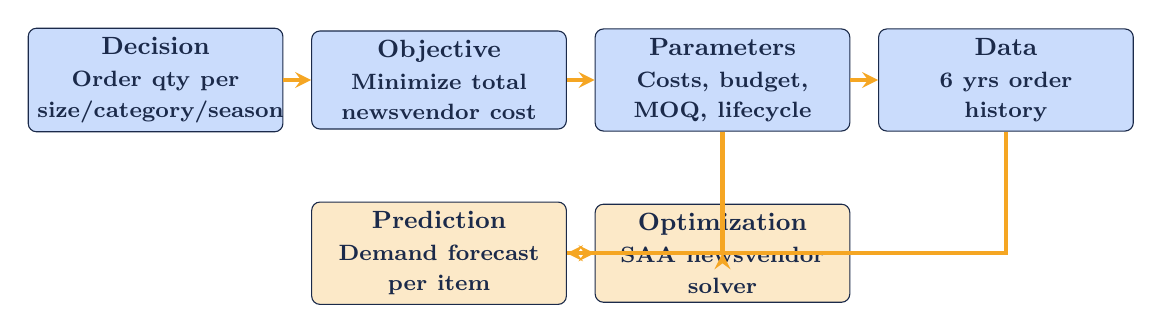
\begin{tikzpicture}[
    box/.style={rectangle, draw=navyblue, fill=iceblue, text=navyblue,
                rounded corners=3pt, minimum width=3.2cm, minimum height=1cm,
                font=\small\bfseries, align=center, text width=3cm},
    arr/.style={->, thick, color=goldyellow, >=stealth, line width=1.5pt}
  ]
  \node[box] (dec) at (0,0)    {Decision\\[2pt]\footnotesize Order qty per\\size/category/season};
  \node[box] (obj) at (3.6,0)  {Objective\\[2pt]\footnotesize Minimize total\\newsvendor cost};
  \node[box] (par) at (7.2,0)  {Parameters\\[2pt]\footnotesize Costs, budget,\\MOQ, lifecycle};
  \node[box] (dat) at (10.8,0) {Data\\[2pt]\footnotesize 6 yrs order\\history};

  \node[box, fill=goldyellow!25] (pred) at (3.6,-2.2) {Prediction\\[2pt]\footnotesize Demand forecast\\per item};
  \node[box, fill=goldyellow!25] (opt) at (7.2,-2.2) {Optimization\\[2pt]\footnotesize SAA newsvendor\\solver};

  \draw[arr] (dec) -- (obj);
  \draw[arr] (obj) -- (par);
  \draw[arr] (par) -- (dat);
  \draw[arr] (dat) |- (pred);
  \draw[arr] (pred) -- (opt);
  \draw[arr] (par) |- (opt);
\end{tikzpicture}

\bigskip
\begin{columns}[T]
\column{0.48\textwidth}
\textbf{Objective:}\\
$\min_{\mathbf{q}} \; \sum_i \bigl[ c_i q_i + \tfrac{1}{S}\sum_s ( o_i [q_i - d_{is}]^+ + u_i [d_{is} - q_i]^+ ) \bigr]$

\column{0.48\textwidth}
\textbf{Constraints:}
\begin{itemize}\small
  \item Budget: $\sum_i c_i q_i \leq B$ per season
  \item MOQ: $q_i \geq 6$ per size
  \item Non-negativity: $q_i \geq 0$
\end{itemize}
\end{columns}
\end{frame}

%% ====================================================================
%% SLIDE 4 -- Data
%% ====================================================================
\begin{frame}{Data: Source and Preparation}

\begin{columns}[T]
\column{0.5\textwidth}
\textbf{Source:} CFA Squarespace order export\\
{\small Proprietary data, authorized by league president}

\medskip
\textbf{Raw:} 90,010 rows $\times$ 52 columns (2017--2026)\\
\textbf{Cleaned:} 12,209 line items $\times$ 10 columns

\medskip
\textbf{Key columns:}\\
{\small order\_date, season, year, product\_category, gender\_age, size, quantity, unit\_price}

\medskip
\textbf{Cleaning challenges:}
\begin{itemize}\small
  \item Size embedded in free-text variant strings
  \item Product names inconsistent across seasons
  \item Lifecycle year must be inferred
  \item Interleaved order-level and line-item rows
\end{itemize}

\column{0.47\textwidth}
\begin{block}{Cleaned Data Profile}
\centering\small
\begin{tabular}{lr}
\toprule
\textbf{Metric} & \textbf{Value} \\
\midrule
Records & 12,209 \\
Date range & 2020--2026 \\
Categories & 3 \\
Size codes & 14 \\
Seasons & 3 (fall/winter/spring) \\
Null columns & 0 \\
\bottomrule
\end{tabular}
\end{block}

\vspace{6pt}
\begin{block}{Train / Test Split}
\small
\textbf{Chronological} (no leakage):\\
Train on historical seasons\\
Test by backtesting against a held-out period\\
{\footnotesize Agent determines optimal split from problem description}
\end{block}
\end{columns}
\end{frame}

%% ====================================================================
%% SLIDE 5 -- Agent Architecture
%% ====================================================================
\begin{frame}{Agent Architecture: 4-LLM-Agent Pipeline}

\centering
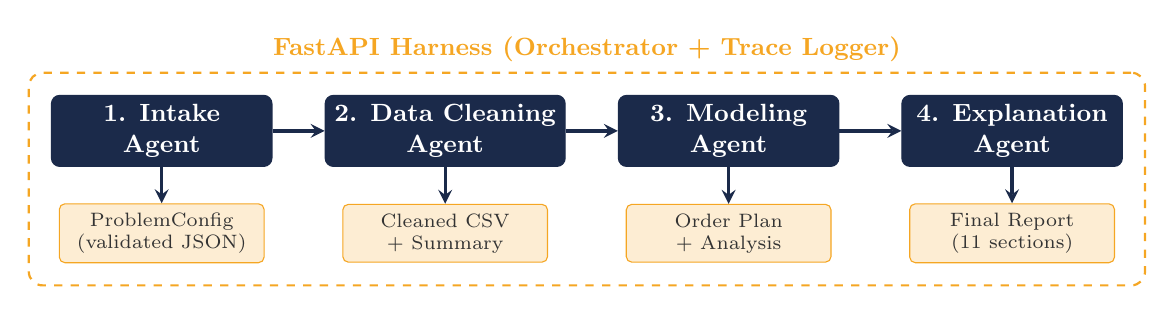
\begin{tikzpicture}[
    agent/.style={rectangle, draw=navyblue, fill=navyblue, text=white,
                  rounded corners=3pt, minimum width=2.8cm, minimum height=0.9cm,
                  font=\small\bfseries, align=center},
    output/.style={rectangle, draw=goldyellow, fill=goldyellow!20, text=darkgray,
                   rounded corners=2pt, minimum width=2.6cm, minimum height=0.55cm,
                   font=\scriptsize, align=center},
    arr/.style={->, thick, color=navyblue, >=stealth, line width=1.2pt}
  ]
  \node[agent] (a1) at (0,0)    {1. Intake\\Agent};
  \node[agent] (a2) at (3.6,0)  {2. Data Cleaning\\Agent};
  \node[agent] (a3) at (7.2,0)  {3. Modeling\\Agent};
  \node[agent] (a4) at (10.8,0) {4. Explanation\\Agent};

  \node[output] (o1) at (0,-1.3)    {ProblemConfig\\(validated JSON)};
  \node[output] (o2) at (3.6,-1.3)  {Cleaned CSV\\+ Summary};
  \node[output] (o3) at (7.2,-1.3)  {Order Plan\\+ Analysis};
  \node[output] (o4) at (10.8,-1.3) {Final Report\\(11 sections)};

  \draw[arr] (a1) -- (o1);
  \draw[arr] (a2) -- (o2);
  \draw[arr] (a3) -- (o3);
  \draw[arr] (a4) -- (o4);
  \draw[arr] (a1) -- (a2);
  \draw[arr] (a2) -- (a3);
  \draw[arr] (a3) -- (a4);

  \node[draw=goldyellow, dashed, thick, rounded corners=5pt,
        fit=(a1)(a2)(a3)(a4)(o1)(o2)(o3)(o4),
        inner sep=8pt, label={[font=\small\bfseries, text=goldyellow]above:FastAPI Harness (Orchestrator + Trace Logger)}] {};
\end{tikzpicture}

\bigskip
\begin{columns}[T]
\column{0.48\textwidth}
\textbf{Design principles:}
\begin{itemize}\small
  \item LLMs at \emph{judgment} touchpoints only
  \item Deterministic Python for all numerics
  \item Sandboxed code execution (agents generate and run Python)
  \item File-based state passing (auditable, replayable)
\end{itemize}

\column{0.48\textwidth}
\textbf{Guardrails:}
\begin{itemize}\small
  \item Pydantic schema validation at every handoff
  \item Budget constraint enforced structurally
  \item Agents write structured summaries, not free-form text
  \item Every step traced in JSON with timing and token usage
\end{itemize}
\end{columns}
\end{frame}

%% ====================================================================
%% SLIDE 6 -- Agent Detail: What Each Does
%% ====================================================================
\begin{frame}{What Each Agent Does}

\begin{columns}[T]
\column{0.48\textwidth}

\begin{block}{1. Intake Agent}
\small
\textbf{Input:} Problem description (NL or file) + CSV\\
\textbf{Tools:} Data inspection (peek, sample, describe, unique values), save\_config\\
\textbf{Output:} Validated ProblemConfig JSON\\
\textbf{Key:} Brainstorms with user, asks clarifying questions, then saves a Pydantic-validated config
\end{block}

\vspace{4pt}
\begin{block}{2. Data Cleaning Agent}
\small
\textbf{Input:} Raw CSV + ProblemConfig\\
\textbf{Tools:} Data inspection, execute\_code (sandbox), save\_summary\\
\textbf{Output:} Cleaned CSV + cleaning summary\\
\textbf{Key:} Generates its own Python cleaning code -- fully generic, no hardcoded logic
\end{block}

\column{0.48\textwidth}

\begin{block}{3. Modeling Agent}
\small
\textbf{Input:} Cleaned CSV + ProblemConfig\\
\textbf{Tools:} load\_data, run\_prediction (tunable), run\_optimization, validate\_results, sensitivity, baseline, execute\_code\\
\textbf{Output:} Order plan + optimizer comparison + summary\\
\textbf{Key:} Inspects data \emph{before} modeling, fixes granularity issues, adds features, tunes hyperparameters
\end{block}

\vspace{4pt}
\begin{block}{4. Explanation Agent}
\small
\textbf{Input:} All run artifacts\\
\textbf{Tools:} read\_file, list\_files, save\_report\\
\textbf{Output:} 11-section final report (Markdown)\\
\textbf{Key:} Writes for dual audience (instructor + business executive)
\end{block}
\end{columns}
\end{frame}

%% ====================================================================
%% SLIDE 7 -- Prediction Methodology
%% ====================================================================
\begin{frame}{Prediction: Methodology}

\begin{columns}[T]
\column{0.55\textwidth}
\textbf{Models compared:}
\begin{itemize}\small
  \item XGBoost (gradient boosting, tunable depth/LR/trees)
  \item LightGBM (leaf-wise growth, fast)
  \item Ridge (linear baseline)
  \item Each model $\times$ PTO-adjusted variant (6 total)
\end{itemize}

\medskip
\textbf{PTO (Predict-then-Optimize):}\\
{\small Shifts predictions by the newsvendor critical ratio:\\
$q^* = \hat{D} \cdot (1 + (CR - 0.5) \cdot \text{strength})$\\
Intentionally biases toward the cost-optimal quantile.}

\medskip
\textbf{Features:} Auto-engineered from data\\
{\small Label-encoded categoricals, year trend, derived features.\\
The modeling agent can add domain features via code.}

\column{0.42\textwidth}
\begin{block}{Why Newsvendor Cost, Not RMSE?}
\small
Following Bertsimas--Kallus (2020):\\[4pt]
Two models with \emph{identical RMSE} can yield very different ordering costs because the newsvendor penalizes errors \textbf{asymmetrically}.\\[4pt]
Under-prediction (stockout) costs up to 5\texttimes{} more than over-prediction.\\[4pt]
$\Rightarrow$ We rank models by the \textbf{realized newsvendor cost} of the orders they imply.
\end{block}

\vspace{4pt}
\begin{block}{Tuning Levers}
\small
Agent can adjust: tree depth, learning rate, estimator count, PTO strength, train/test years
\end{block}
\end{columns}
\end{frame}

%% ====================================================================
%% SLIDE 8 -- Optimization Methodology
%% ====================================================================
\begin{frame}{Optimization: Methodology}

\textbf{Formulation:} Sample Average Approximation (SAA) of the multi-product newsvendor

$$\min_{\mathbf{q}} \; \sum_{i=1}^{N} \left[ c_i q_i + \frac{1}{S}\sum_{s=1}^{S} \left( o_i (q_i - d_{is})^+ + u_i (d_{is} - q_i)^+ \right) \right]$$

\medskip
\begin{columns}[T]
\column{0.48\textwidth}
\textbf{Five solvers benchmarked:}
\begin{enumerate}\small
  \item \textbf{SLSQP} -- sequential quadratic programming
  \item \textbf{L-BFGS-B} -- quasi-Newton, box-constrained
  \item \textbf{Projected Gradient Descent} -- first-order, projected
  \item \textbf{SGD} -- stochastic gradient descent
  \item \textbf{Adam} -- adaptive moment estimation
\end{enumerate}

\medskip
{\small Multiple random restarts to handle non-convexity in the multi-product case.}

\column{0.48\textwidth}
\textbf{Constraint handling:}
\begin{itemize}\small
  \item Budget: hard constraint via SLSQP, projection step for first-order methods
  \item MOQ: floor projection ($q_i \geq 6$)
  \item Non-negativity: box bounds
\end{itemize}

\medskip
\textbf{What the modeling agent checks:}
\begin{itemize}\small
  \item All solvers feasible?
  \item Budget binding or slack?
  \item Realized cost vs.\ expected cost
  \item Sensitivity to cost parameters
  \item Agent plan vs.\ naive baseline
\end{itemize}
\end{columns}
\end{frame}

%% ====================================================================
%% SLIDE 9 -- Adaptability
%% ====================================================================
\begin{frame}{Adaptability: What Can the Instructor Change?}

\begin{columns}[T]
\column{0.48\textwidth}
\begin{block}{Handled by Re-Run (config change only)}
\small
\begin{itemize}
  \item New constraint\\{\footnotesize ``Add a sustainability cap of 500 total units''}
  \item Changed costs\\{\footnotesize ``Rush shipping now costs 2\texttimes{} more''}
  \item Different budget\\{\footnotesize ``Budget is \$12,000 not \$8,000''}
  \item New season of data\\{\footnotesize Drop in updated CSV, re-run pipeline}
  \item Shifted objective\\{\footnotesize ``Maximize service level instead''}
\end{itemize}
\end{block}

\column{0.48\textwidth}
\begin{block}{Needs Re-Engineering}
\small
\begin{itemize}
  \item Fundamentally different problem class\\{\footnotesize e.g., staff scheduling instead of inventory}
  \item New data source not in existing dataset
  \item Structurally new constraint types\\{\footnotesize e.g., per-team allocation, tiered discounts}
\end{itemize}
\end{block}

\vspace{6pt}
\textbf{How it works:}\\
{\small User changes a field in ProblemConfig (via chat or JSON edit) $\rightarrow$ pipeline re-runs automatically $\rightarrow$ new order plan in ${\sim}$10 minutes.}
\end{columns}
\end{frame}

%% ====================================================================
%% SLIDE 10 -- Live Demo
%% ====================================================================
\begin{frame}{Live Agent Demo}

\vfill
\centering
{\Large\bfseries\color{navyblue} Live Demonstration}

\bigskip
{\large
1. Upload CSV and problem description\\[4pt]
2. Brainstorm with the Intake Agent\\[4pt]
3. Approve the ProblemConfig\\[4pt]
4. Watch the pipeline run:\\
\quad Data Cleaning $\rightarrow$ Modeling $\rightarrow$ Explanation\\[4pt]
5. View the final report with order plan
}

\bigskip
\begin{block}{}
\centering
\textit{We will demonstrate a stakeholder modification --\\
the instructor may change a constraint or cost parameter mid-demo.}
\end{block}
\vfill
\end{frame}

%% ====================================================================
%% SLIDE 11 -- Results (filled during/after demo)
%% ====================================================================
\begin{frame}{Results from Demo Run}

\vfill
\centering
{\large\color{navyblue}\bfseries Results populated from live demo}

\bigskip
\begin{columns}[T]
\column{0.32\textwidth}
\begin{block}{Prediction}
\centering\small
Best model: \rule{2cm}{0.4pt}\\
NV cost: \rule{2cm}{0.4pt}\\
vs.\ baseline: \rule{2cm}{0.4pt}
\end{block}

\column{0.32\textwidth}
\begin{block}{Optimization}
\centering\small
Best solver: \rule{2cm}{0.4pt}\\
Total spend: \rule{2cm}{0.4pt}\\
Budget feasible: \rule{2cm}{0.4pt}
\end{block}

\column{0.32\textwidth}
\begin{block}{Business Impact}
\centering\small
Cost savings: \rule{2cm}{0.4pt}\\
vs.\ current process: \rule{2cm}{0.4pt}\\
Confidence: \rule{2cm}{0.4pt}
\end{block}
\end{columns}

\bigskip
{\small\color{darkgray} The Explanation Agent generates a full 11-section report with\\
order table, sensitivity analysis, and baseline comparison.}
\vfill
\end{frame}

%% ====================================================================
%% SLIDE 12 -- Managerial Takeaways
%% ====================================================================
\begin{frame}{Managerial Takeaways}

\begin{enumerate}
  \item \textbf{The agent produces a budget-feasible, cost-minimizing order plan} --
        something the current ``gut feel'' process cannot guarantee.

  \item \textbf{Focus attention on youth jerseys} -- they drive the majority of spend
        and carry the most forecasting risk. Adult/women sizes are set by MOQ.

  \item \textbf{The budget is the binding constraint} -- not the forecast model.
        If the budget is too tight, no algorithm can prevent stockouts.

  \item \textbf{Cost estimates matter more than demand accuracy} -- the plan is
        highly sensitive to underage cost assumptions and nearly flat to overage.

  \item \textbf{Re-run the agent when conditions change:} new cost data, updated budget,
        new season of orders, jersey model transition.

  \item \textbf{The system is generic} -- the same pipeline can optimize any
        newsvendor-class inventory problem, not just soccer uniforms.
\end{enumerate}
\end{frame}

%% ====================================================================
%% SLIDE 13 -- Limitations & Future Work
%% ====================================================================
\begin{frame}{Limitations \& Future Work}

\begin{columns}[T]
\column{0.48\textwidth}
\textbf{Current limitations:}
\begin{itemize}\small
  \item Demand at the size level is inherently noisy -- tail spikes are not predictable from order history alone
  \item Sparse data for rare sizes (AXL, WXL) -- MOQ dominates these cells
  \item Jersey carryover inventory not yet modeled as a constraint
  \item Pipeline runtime ${\sim}$10 min (dominated by optimizer solver)
\end{itemize}

\column{0.48\textwidth}
\textbf{Future improvements:}
\begin{itemize}\small
  \item \textbf{Registration/roster data} as a leading demand indicator
  \item \textbf{Hierarchical models} to borrow strength across sparse sizes
  \item \textbf{Carryover-net ordering} as a first-class constraint
  \item \textbf{End-to-end prescriptive model} (Bertsimas--Kallus) training directly on newsvendor loss
  \item Interactive config editor in the web UI
\end{itemize}
\end{columns}

\bigskip
\centering
\begin{block}{}
\centering\small
\textbf{Adaptable:} any change expressible in ProblemConfig fields.\\
\textbf{Transparent:} every agent writes a structured summary; full trace logged.\\
\textbf{Testable:} benchmark problems can be fed as problem description files.
\end{block}
\end{frame}

%% ====================================================================
%% SLIDE 14 -- Q&A
%% ====================================================================
\begin{frame}[standout]
\vfill
{\Huge Questions?}

\bigskip
{\large Thank you!}

\bigskip
{\normalsize
Satya Ganteda \;\textbar\;
Daniel Affleck \;\textbar\;
Siddharth Shenoy \;\textbar\;
Fabian Macias \;\textbar\;
Aditya Gupta
}

\medskip
{\small MGMT 590-037 -- AI-Enhanced Optimization -- Summer 2026}
\vfill
\end{frame}

\end{document}
